\documentclass{article}

\usepackage{amsmath}
\usepackage{graphicx}
\usepackage{dsfont}

\DeclareGraphicsExtensions{.pdf, .png, .jpg}

\setcounter{secnumdepth}{0}

\title{Design Document}
\author{Alexandra Anderson (aea84), Nerla Jean-Louis (nj99)}
\date{May 6, 2015}

\begin{document}
\maketitle



%\begin{figure}[h]
%	\includegraphics[width = \textwidth]{pipeline}
%	\caption{The packet processing pipeline.}
%end{figure}

\section{Pipeline and Parallelism}

See the figure at the end of the document for a diagram of the pipeline and a description of what each stage does. 

We plan to use a minimally pipelined and extremely parallelized system. The two performance bottlenecks potentially are the hash computation, and lock competition. The hash computation cannot be usefully pipelined, so we reserve most of our cores for that work. Instead of looking up the evil list right there, the hash result is stored with the packet. 

In order to minimize lock competition, we place the most complicated data structures in pipeline stages executed by only one core. The stages are connected by shared lists, which do have lock competition. However, a list is both simpler to lock and requires locks to be held for far shorter times. The obvious implementation to keep track of spam, vulnerable, and evil packet statistics is with a hashtable, and in case of parallelism the entire table would need to be locked. Instead, we designate one thread in a stage where the primary task is accessing those hashtables, without need for locking.

We also plan to test dividing that stage into multiple, as a way of allocating more threads to the tail end of computation, but we do not expect that to be a bottleneck. 

\section{Shared and Isolated Data Structures}

We have a shared linked list queue structure which is lockable, and uses a mutex for both adding and polling. Only one thread should be able to read or modify the list at once.

We will also have an unlocked hash table structure, which is only ever accessed by the one thread in that stage of the pipeline. The space necessary for possible table expansions is pre-allocated upon initialization of the network device, but we begin with a smaller buffer in order to facilitate scanning and printing the entire list of evil, spam, vulnerable ports. 

\subsection{Packet Organization}
Each packet is stored in a sigle page of memory. We store a lock, hash-value, a pointer to the packet and a pointer to the next packet in the extra 68 bytes of space in the page.

\subsection{Linked Lists}SFTP

Each pipeline stage has a linked list containing all of the packets currently in that stage. Each pipeline stage has a header struct that contains a lock so only one core can remove a packet from the list at a time and one can add to the list at a time.

\begin{figure}[h]
	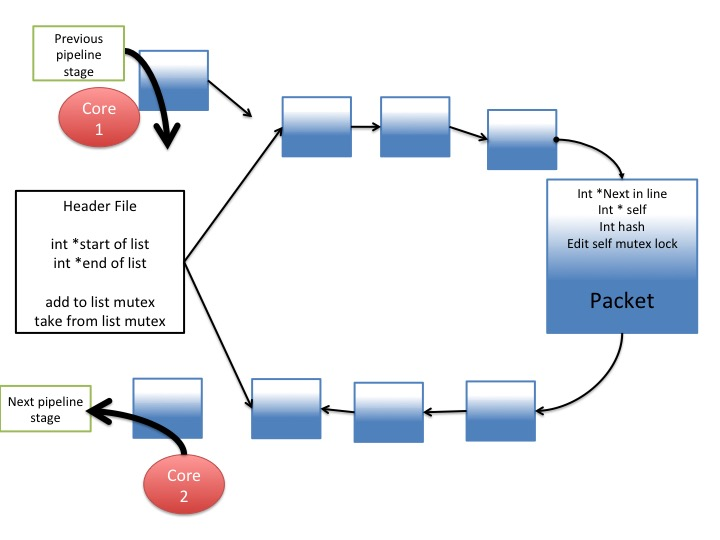
\includegraphics[width = \textwidth]{Slide1}
	\caption{Shared Data Structure Linked List}
\end{figure}

\section{Memory Management}

In order to avoid synchronizing malloc, we allocate all 12MB of memory upon startup. Packets are allocated as 4KB pages, which gives 4000 bytes of data, 28 bytes of network header, and leaves 68 bytes per packet for containing our generated header information. This means that the packets are page-aligned, reducing the need for transferring pages to and from the disk while processing a single packet. 

We also initially allocate memory for the data structures containing the vulnerable, spam, and evil lists. While we will experiment to see how much memory is ideal, we anticipate allocating around 4-6MB. This will ensure that even with bloated lists, the threshold for dropping commands is very low.

We still retain 6-8MB for packets, which translates to 1536 to 2048 different packets that can be in the system at once before packets drop due to lack of memory. 

\end{document}